% -*- coding: utf-8; -*-

\chapter{Introduction}
There are several reasons that motivate the adoption of statically typed languages. Maintaining large systems built with dynamic types can become a nightmare due to the lack of type information \cite{takikawa_is_2016}. Typed languages also generally has better performance because compile-time type information helps generating optimized machine code. However, programmers are left empty handed when faced with re-writing code from a dynamically typed language to a statically typed one. Most of the times they have to re-write the entire system if gradually typed languages are not an option.
\newline
In order to aid programmers to understand the relationship of the types between parts of a program we decided to build a dynamic type extractor for the Lua programming language. The Type Extractor will give you information about function types in a program inspected during runtime. With this information programmers can more easly migrate to a statically typed language. The information generated by our Type Extractor can also be used for code inspection and serve as an useful documentation.
\newline
This software is destinated for programmers who wants to understand the existing types within their Lua programs, developers aiming to produce a useful documentation and also to inspect the type behaviour of variables and functions present in their code.



% \begin{figure}
% \centering
% 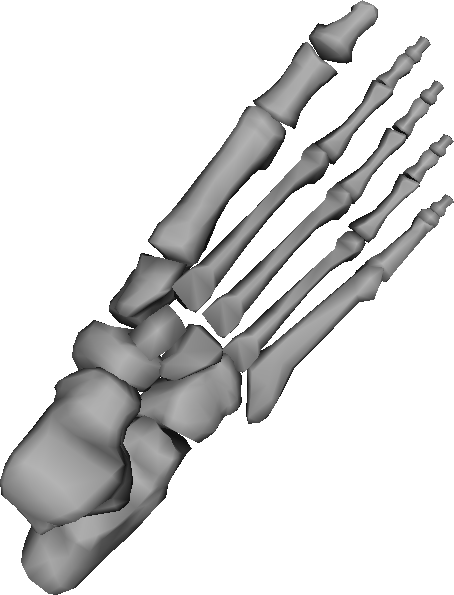
\includegraphics[width=0.45\textwidth]{pictures/image01.png}
% 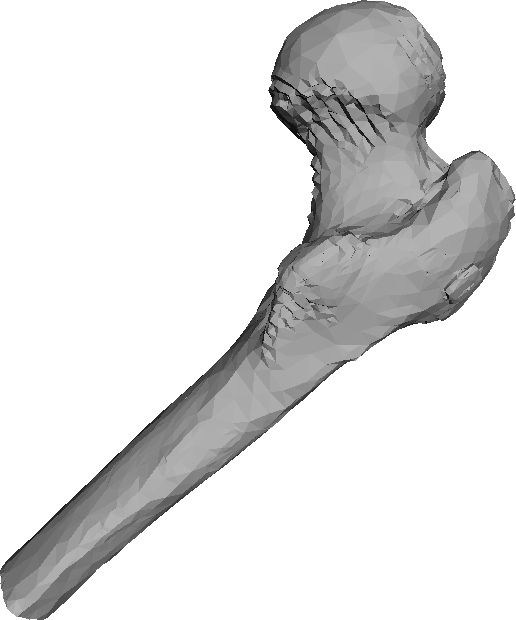
\includegraphics[width=0.45\textwidth]{pictures/image02.png}
% \caption{Meshes generated from medical data. Data obtained from the AIM$@$SHAPE Shape Repository \cite{AIMSHAPE}}
% \label{fig:example}
% \end{figure}

%This document is structured as follows. In Chapter~\ref{cha:Previous Work} we present some previous work relevant to our problem. In Chapter~\ref{cha:Proposal} we explain our proposal. In Chapter~\ref{cha:Results} we show our results. Finally, in Chapter~\ref{cha:Conclusion} we present our conclusion and future work.


